\documentclass[11pt]{article}

\usepackage[margin=1in]{geometry}
\usepackage{amsmath,amssymb}
\usepackage{array}
\usepackage{booktabs}
\usepackage{enumitem}
\usepackage{xcolor}
\usepackage{hyperref}
\usepackage{setspace}
\usepackage{float}
\usepackage{graphicx}
\usepackage{tikz}
\usetikzlibrary{arrows.meta,positioning,fit}

\setstretch{1.10}
\setlength{\emergencystretch}{2em}

\hypersetup{
    colorlinks=true,
    linkcolor=blue!50!black,
    urlcolor=blue!50!black,
    citecolor=black
}

% Draft markers: every \todo must be resolved or deleted before submission.
\newcommand{\todo}[1]{\textcolor{red}{[TODO: #1]}}

% --------------------
% Course information
% --------------------
\newcommand{\course}{DSA4213: Natural Language Processing for Data Science}
\newcommand{\semester}{Semester 1, AY2026/2027}

\graphicspath{{../results/}}

\begin{document}

\begin{center}
{\LARGE\bfseries Group Project Final Report}\\[0.4em]
{\large Interruptible MLE Agents: Human Intervention in Long-Horizon Tree Search}\\[0.9em]
Group ID: Group 7\\[0.9em]
\course\\
\semester
\end{center}

% ====================
% Administrative information
% ====================
\section*{Administrative Information}

\begin{tabular}{@{}>{\bfseries\raggedright\arraybackslash}p{0.25\linewidth}
                    >{\raggedright\arraybackslash}p{0.70\linewidth}@{}}
Group members & Nabil Rakaiza Abror (A0305715J) \\
               & Dziand Dafi Ginandjar (A0354009J) \\
               & Medhini Karthikeyan (A0351868N) \\
               & Sahishnav Kritin Karamarathur Senthil Kumar (A0357345X) \\[0.7em]
Project direction & Human-in-the-loop, tool-using agents for machine learning
                    engineering. \\[0.7em]
Repository & \url{https://github.com/nabilrakaiza/interruptible-mle-agent} \\
\end{tabular}

% ====================
% Executive summary
% ====================
\section*{Project Summary}

MLE agents steer a long search with a validation score they compute themselves, and
prior work shows this score drifts away from held-out performance. We built a
tree-search MLE agent that a human can interrupt: it shows its tree, its findings and a
hidden \emph{probe} score on a dashboard, and applies structured interventions at safe
points between nodes. A separate evaluation agent (A1) writes the splits and scoring
harness once, and the coding agent cannot change them. We ran 118 four-hour runs on six
MLE-bench Lite tasks (text, tabular, image), comparing an autonomous baseline (C1: the
full agent with no monitor), two scripted policies that stand in for a monitoring human,
and two ablations, and analysed the 63 runs on the three text tasks in depth. No
condition beat C1 (Friedman $p = 0.55$ over task $\times$ seed blocks on the text tasks;
no task separates them). With A1 in place, the drift the interventions target barely
occurred; without it, validation was more optimistic on the text tasks and nomad, and 2
of 17 runs leaked. The differences between tasks are consistent with the size of the
held-out splits. Five live human sessions changed no outcome beyond noise; as a design
implication, they suggest a person's input would matter most as task knowledge and a
direct instruction channel rather than score-watching.

% ====================
% 1. Problem and motivation
% ====================
\section*{1. Problem, Research Question, and Motivation}

\begin{quote}
\textbf{Which human interventions into a tree-search MLE agent improve its outcomes,
and at what interaction cost?}
\end{quote}
\vspace{-0.3em}
Two sub-questions follow: \emph{can a human, given a progress view, detect and correct
the validation--test divergence that the agent cannot see?}, and \emph{does it matter
whether an intervention changes the agent's next action} (prune, redirect, override)
\emph{or its beliefs} (inject knowledge, correct a stored finding)?

\textbf{Motivation.} Toledo et al.\ \cite{aira} found that an agent's cross-validation
score keeps climbing over a 24-hour run while its test score plateaus, and that picking
the final node by test instead of validation would raise the medal rate by 9 to 13
points. The failure is invisible from inside the loop: in MLE-STAR \cite{mlestar},
validation accuracy on \texttt{spaceship-titanic} rose from 0.819 to 0.868 while test
accuracy fell from 0.803 to 0.734 because generated features used the target. Yet the
published MLE agents \cite{aide,aira,mlestar,mlmaster,mlmaster2} are autonomous by
construction and give a human no way in. An agent-based approach is needed because the
search space is the space of programs, with no predefined space for AutoML
\cite{aide}: the system interleaves reasoning with execution feedback \cite{react},
searches candidates with a verifier \cite{tot} and acts through a constrained interface
\cite{sweagent}, and the question arises only because it makes hundreds of
consequential decisions unsupervised. The intended setting is a practitioner who leaves
an MLE agent running for hours and wants to oversee it, not do the work by hand.

\textbf{Success} meant an interruptible agent with valid submissions on most tasks, a
documented intervention vocabulary, a controlled comparison and reproducible artefacts.
The first three were met and the fourth in part: run folders contain competition data,
so only their summaries are public. Beating the state of the art was not a goal.

\textbf{Changes since the proposal.} Each member ran the plan on their own task(s):
the full 21-run plan on five tasks and a 13-run half plan on cactus, with insults and
pizza on Kaggle CPUs without Docker. C4's thresholds came from pilot replays and C5's
were fixed in advance, so the live sessions (none on pizza) were compared against the
rules instead of used to write them. To spend compute and time on seeds we did not run
A2-off, the exploration-diversity metric or the contamination spot-check, and A1's leak
screen uses static rules instead of an LLM judgement. Two LLM-monitor runs sit outside
the study (Appendix F).

% ====================
% 2. Related work and contribution
% ====================
\section*{2. Related Work and Contribution}

MLE-bench \cite{mlebench} turns 75 Kaggle competitions into offline tasks with the
original medal thresholds; we use its 22-task Lite subset. AIDE \cite{aide} searches over
scored Python scripts grown by draft, debug and improve operators. AIRA-dojo \cite{aira}
varies these components one at a time and documents the proxy-metric overfitting
above. MLE-STAR \cite{mlestar} adds web retrieval of candidate models and leakage
checkers. ML-Master \cite{mlmaster,mlmaster2} adds MCTS and a hierarchy of distilled
findings, close to the reflections of Generative Agents \cite{genagents}. For general
agents, AGDebugger \cite{agdebugger} adds rollback and message editing, and
Magentic-UI \cite{magentic} co-planning and action approval; neither handles a search
over scored programs, where interruption must respect long-running training jobs.

\textbf{Contribution.} The tree and operators follow AIDE, the findings ML-Master 2.0,
and the leakage screen MLE-STAR. Beyond these, we contribute (1)
\textbf{interruptibility as a property of the search loop}: safe-point checkpoints, an
intervention queue shared by humans and scripted policies, a dashboard with a hidden
probe score, and run replay; (2) \textbf{a measurement of intervention value in MLE}
over 118 controlled runs on six tasks plus five live human sessions; (3) \textbf{structural separation of
evaluation from optimisation}, enforced by the environment, stress-tested and
ablated; and (4) \textbf{a well-supported negative result} with an explanation
(Section 6). We use MLE-bench's data preparation and graders, DeepSeek V4 Flash 0731
\cite{deepseek} through OpenRouter \cite{openrouter}, Docker \cite{docker}, Streamlit
\cite{streamlit}, and scikit-learn \cite{sklearn} and PyTorch \cite{pytorch} in the
sandbox.

% ====================
% 3. Agent setup
% ====================
\section*{3. Agent and Task Setup}

\textbf{Task and environment.} Given a competition description and data, the system
writes \texttt{submission.csv}, graded by MLE-bench. Each run has 4 hours, 2 CPUs, a
20-minute limit per script and a 200-node cap. Scripts ran CPU-only in a Docker sandbox (4\,GB, no
network) on each member's laptop, or in a subprocess sandbox on Kaggle for insults and
pizza (machines in Appendix J). All LLM calls use DeepSeek V4 Flash 0731 (fp8) at temperature 0.7.

\textbf{Sub-agents.}
\textbf{A1 (evaluation)} runs once: it splits the labelled data into training,
validation and a 10\% \emph{probe} split with a fixed seed, so all runs on a task share
identical splits, writes the scoring harness and freezes it. Before execution it
screens each script with static rules for reading outside the input folder, the
target among the features, statistics fitted on prediction rows, and validation rows
used for fitting. \textbf{A2 (retrieval)} returns up to 8 model cards from allowlisted
library documentation; solution sites are blocked. \textbf{A3 (coding)} implements draft, debug and improve, each a plan plus a
self-contained script that trains, scores itself through the harness and predicts the
test set. \textbf{A4 (reflection)} writes up to 3 findings every 10 nodes, each citing
its nodes and scores; the 10 newest are shown to A3. \textbf{A5 (controller)}, not an
LLM, selects the next node and operator, enforces stopping rules, checkpoints and
applies interventions; it is the only writer to the tree. Permissions are enforced by
the environment, not prompts (Appendix~I): A3 can neither modify the harness nor reach
the network. The probe score is never shown to A3 or used
by A5; every node's test score is graded for analysis but never shown to any agent.
\textbf{Interruption semantics.} A \emph{safe point} is a node boundary, after a script
has been scored and before A5 selects the next node. There A5 checkpoints the tree,
findings, harness, budget and random state, and drains an intervention queue:
\emph{action} interventions (\textbf{prune} a subtree, \textbf{redirect} the next node
and operator, \textbf{override} the final pick), \emph{belief} interventions
(\textbf{inject} a model card, \textbf{correct} or delete a finding) and
\textbf{rebudget}. The clock keeps running while a human thinks, so all runs get equal
time, and every action is logged with its time, target and note.
\textbf{Stopping}: a run ends at the budget or node cap; a debug chain stops after 3
failures and an improve chain after 3 attempts without a 0.1\% relative gain.

% ====================
% 4. System or study design
% ====================
\section*{4. System and Study Design}

\begin{figure}[tb]
\centering
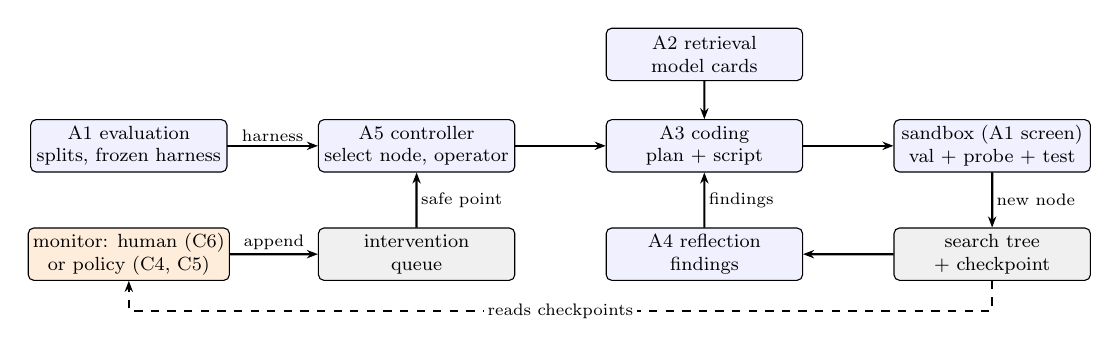
\begin{tikzpicture}[scale=0.86, transform shape,
  box/.style={draw, rounded corners=2pt, align=center, font=\footnotesize,
              minimum height=2.2em, minimum width=2.9cm, inner sep=2pt},
  agent/.style={box, fill=blue!6},
  store/.style={box, fill=gray!12},
  human/.style={box, fill=orange!14},
  arr/.style={-{Stealth[length=4pt]}, thick},
  lab/.style={font=\scriptsize, inner sep=1.5pt}]
  \node[agent] (a1) at (0,0)    {A1 evaluation\\ splits, frozen harness};
  \node[agent] (a5) at (4.25,0)  {A5 controller\\ select node, operator};
  \node[agent] (a3) at (8.5,0)  {A3 coding\\ plan + script};
  \node[agent] (sb) at (12.75,0) {sandbox (A1 screen)\\ val + probe + test};
  \node[agent] (a2) at (8.5,1.35) {A2 retrieval\\ model cards};
  \node[human] (mon) at (0,-1.6) {monitor: human (C6)\\ or policy (C4, C5)};
  \node[store] (q)  at (4.25,-1.6) {intervention\\ queue};
  \node[agent] (a4) at (8.5,-1.6) {A4 reflection\\ findings};
  \node[store] (tr) at (12.75,-1.6) {search tree\\ + checkpoint};
  \draw[arr] (a1) -- node[lab,above]{harness} (a5);
  \draw[arr] (a5) -- (a3);
  \draw[arr] (a2) -- (a3);
  \draw[arr] (a3) -- (sb);
  \draw[arr] (sb) -- node[lab,right]{new node} (tr);
  \draw[arr] (tr) -- (a4);
  \draw[arr] (a4) -- node[lab,right]{findings} (a3);
  \draw[arr] (mon) -- node[lab,above]{append} (q);
  \draw[arr] (q) -- node[lab,right]{safe point} (a5);
  \draw[arr, dashed] (tr.south) -- ++(0,-0.45) -| node[lab,pos=0.25,fill=white]{reads checkpoints} (mon.south);
\end{tikzpicture}
\caption{System overview. The agent process is the only writer to the tree. The
dashboard and scripted policies run as separate processes that read checkpoints and
append to the queue, so human and scripted interventions take the same code path.}
\label{fig:system}
\end{figure}

\textbf{Main loop} (Figure~\ref{fig:system}). A5 picks a node and operator greedily on
validation (5 drafts, 50\% debug chance, 15\% random improves); A3 writes a script; A1
screens and scores it; A5 applies queued interventions. The best validation node is
submitted.

\textbf{Design choices.} A1's harness is immutable to A3 by file permission, so the agent
cannot score itself on data it trains on unless A1 is switched off. The probe is hidden
so the monitor has a signal the agent never optimises against: a gap between validation
and probe can reveal overfitting the agent cannot see. Scripted policies stand in for a
human because they are reproducible across seeds, whereas a recorded human action
points to a different node on any rerun of a nondeterministic agent.

\textbf{Conditions} (Table~\ref{tab:conditions}) change one component each. C2 and C3
need no runs: every node keeps its graded test score, so both come from C1's trees.

\begin{table}[tb]
\centering
\small
\begin{tabular}{@{}llp{0.6\linewidth}l@{}}
\toprule
\textbf{ID} & \textbf{Condition} & \textbf{What changes} & \textbf{Seeds} \\
\midrule
C1 & Autonomous & Greedy search, best-validation submission. & 0--4 \\
C2 & Oracle pick & C1's best node on test: upper bound on selection. & post hoc \\
C3 & Top-3 & Best of C1's top 3 nodes by validation \cite{aira}. & post hoc \\
C4 & Divergence prune & \emph{Action.} Prune a lineage once validation has improved
      by ${\geq}1\%$ while the probe got ${\geq}1\%$ worse over ${\geq}2$ nodes since
      its best-probe node, in ${\geq}95\%$ of paired bootstrap resamples. & 0--4 \\
C5 & Finding correction & \emph{Belief.} Delete a finding once half of its cited
      nodes gained more than 0.02 more on validation than on the probe. & 0--4 \\
C6 & Live human & A group member watches one live 2-hour run on the dashboard and can
      intervene; one session per task, none on pizza. & 100 \\
\midrule
A1-off & No evaluation agent & A3 writes its own split and metric. & 0--2 \\
A4-off & No reflection & No findings in A3's prompt. & 0--2 \\
\bottomrule
\end{tabular}
\caption{Conditions. C4 and C5 are scripted monitors that use the same queue as a
human.}
\label{tab:conditions}
\end{table}

% ====================
% 5. Evaluation
% ====================
\section*{5. Evaluation and Results}

\textbf{Protocol.} Six MLE-bench Lite tasks: spooky author identification (log loss,
lower is better), insults and pizza (AUC) on text, nomad (RMSLE) on tabular data, and
leaf (log loss) and cactus (AUC) on images. Each full-plan task has 21 runs
(C1, C4, C5 on seeds 0--4; A1-off, A4-off on seeds 0--2) and cactus 13 (seeds 0--2 and
0--1), all at 4 hours with the same model and CPUs: 118 runs. We report MLE-bench's
outcomes (valid, above median, medal) and test score, and three process metrics: the
pick's validation--test gap, probe fidelity (rank correlation of probe and test over a
run's nodes) and selection loss (pick versus the run's best node on test). With 3 to 5
seeds per cell we do not rank conditions whose intervals overlap; across tasks we use a
Friedman test with task $\times$ seed blocks. The in-depth analysis uses the 63
text-task runs, whose run folders we hold; for the others we use each owner's summaries.

\textbf{Outcomes.} All 63 runs made a valid submission above the median
(Table~\ref{tab:outcomes}): insults is gold on 21 of 21 runs, pizza bronze on 9, spooky
bronze on 1. Table~\ref{tab:claims} answers each claim the proposal tied to a
comparison.

\begin{table}[tb]
\centering
\footnotesize
\begin{tabular}{@{}lccccc@{}}
\toprule
\textbf{Condition} & \textbf{Spooky} $\downarrow$ & \textbf{Insults} $\uparrow$
& \textbf{Pizza} $\uparrow$ & \textbf{Medals} & \textbf{Rate [95\% CI]} \\
\midrule
C1 & 0.3290 $\pm$ 0.033 & 0.9019 $\pm$ 0.005 & \textbf{0.6978} $\pm$ 0.010 & 9 of 15 & 60\% [33, 87] \\
C2 (oracle) & 0.3284 $\pm$ 0.034 & 0.9078 $\pm$ 0.001 & 0.7037 $\pm$ 0.007 & 10 of 15 & 67\% \\
C3 (top 3) & 0.3288 $\pm$ 0.033 & 0.9019 $\pm$ 0.005 & 0.6983 $\pm$ 0.009 & 9 of 15 & 60\% \\
C4 & 0.3345 $\pm$ 0.027 & 0.9054 $\pm$ 0.004 & 0.6851 $\pm$ 0.019 & 7 of 15 & 47\% [20, 73] \\
C5 & \textbf{0.3133} $\pm$ 0.023 & 0.9074 $\pm$ 0.006 & 0.6847 $\pm$ 0.011 & 7 of 15 & 47\% [20, 73] \\
A1-off & 0.3592 $\pm$ 0.043 & 0.9062 $\pm$ 0.006 & 0.6851 $\pm$ 0.013 & 4 of 9 & 44\% [11, 78] \\
A4-off & 0.3424 $\pm$ 0.019 & \textbf{0.9107} $\pm$ 0.002 & 0.6818 $\pm$ 0.026 & 4 of 9 & 44\% [11, 78] \\
\midrule
Median / bronze & 0.4188 / 0.2938 & 0.7784 / 0.7911 & 0.5996 / 0.6921 & & \\
\bottomrule
\end{tabular}
\caption{Mean $\pm$ SD of test score over seeds per condition and task; medals pooled
over tasks, with bootstrap intervals over runs. Per-task medals are in Appendix A.}
\label{tab:outcomes}
\end{table}

\begin{table}[tb]
\centering
\small
\begin{tabular}{@{}p{0.29\linewidth}p{0.52\linewidth}p{0.13\linewidth}@{}}
\toprule
\textbf{Claim (proposal)} & \textbf{Evidence (spooky / insults / pizza)} & \textbf{Verdict} \\
\midrule
The agent overfits its own proxy metric & Pick's test minus validation with A1 (median):
  $-0.006$ / $-0.001$ / $-0.021$ & Only pizza \\
The probe is a usable signal & Probe--test rank correlation 0.97 / 0.59 / 0.28
  (validation: 0.98 / 0.55 / 0.53) & Depends on task \\
A human-style policy corrects drift & C4 within seed noise of C1 on every task; its
  rule never changed a pick; C2 caps any selection gain at 0.0006 / 0.006 / 0.006 & No \\
Judgement beats a blind hedge & C3 gains at most 0.0005; C4 is no better beyond
  noise & No \\
Action and belief differ & C4 fired live on 2 of 15 runs; no C5 correction changed a
  pick & Not testable \\
Evaluation separation matters & A1-off gap $-0.088$ / $-0.015$ / $-0.045$; 2 of 17
  A1-off runs leaked (all tasks) & Yes \\
Accumulated findings help & A4-off best on insults, worst on pizza; 61\% of findings
  supported & Not shown \\
Interventions are worth their cost & No C4/C5 action changed a pick; 29 human actions,
  no gain beyond noise & Not testable \\
\bottomrule
\end{tabular}
\caption{Each claim from the proposal's evaluation plan, with the evidence and our
verdict. Gaps are the pick's test minus validation score, oriented so that negative means
validation was optimistic.}
\label{tab:claims}
\end{table}

\subsection*{5.1 Comparisons and Ablations}

\textbf{No condition is clearly better.} The best condition differs by task (C5 on
spooky, A4-off on insults, C1 on pizza), and one condition's own seeds vary more than
the gaps between conditions (spooky: 0.037 to 0.082 within a condition, at most 0.046
between means). Friedman tests find no difference among C1, C4 and C5 ($\chi^2 = 1.2$,
$p = 0.55$, 15 task $\times$ seed blocks) or among all five run conditions ($\chi^2 = 2.2$, $p = 0.69$,
9 task $\times$ seed blocks). The strongest hint, pizza's C1 (4 bronze of 5 against 5 of 16), favours
no intervention.

\textbf{Selection costs little (C2, C3).} The pick is a median 0.000, 0.003 and 0.009
below the run's best node on test; the top-3 hedge recovers at most 0.0005, and picking
by the probe is never better on average (Appendix B).

\textbf{The interventions rarely fired.} Live C4 fired only on pizza (3 prunes in 2
runs); live C5 made 13 corrections (2 spooky, 11 pizza). None changed a final pick.
Replayed on the 48 runs without C4, the C4 rule fires on 11 (8 pizza, 3 spooky): the
pick improves on 3, is unchanged (within 0.0001) on 3 and gets worse on 5, by up to 0.024.

\textbf{A1 keeps validation honest (A1-off).} Without A1 the pick's validation is more
optimistic on every text task (median gap $-0.088$, $-0.015$, $-0.045$ against $-0.006$,
$-0.001$, $-0.021$), and 2 of the 17 A1-off runs across all tasks leaked (spooky and
leaf; Section 6). A1-off changes more than the screen: the agent also writes its own
split and metric, so the ablation tests the whole separation. With A1 no text-task run
leaked, and on all 18 spooky runs the pick's test stays within 0.015 of validation. A1's screen stopped 3
real scripts that trained on validation rows, and in a stress test it flagged 4 of 4
planted leaks, one per rule, and 0 of 4 clean controls.

\textbf{The other three tasks} (Table~\ref{tab:tasks}; Appendices G--H) repeat the
pattern: no condition separates. On nomad 4 runs produced no working node (likely
Docker/WSL2 timeouts) and all 17 valid runs medalled. Without A1, nomad's
validation was again more optimistic (pick gap $-0.0047$ against $-0.0004$) and ranked
nodes almost unlike test (rank correlation 0.09 against 0.67). Cactus is a ceiling task
(every node near AUC 0.9999, a medal needs 1.0); A1-off did not leak, and A1's screen
stopped 4 late stacking scripts fitted on validation rows. Leaf is the one task where selection lost much:
C1's mean log loss is 0.085 against 0.0075 for C2, with 178 validation rows for 99
species. Leaf's A1-off run
at 15.66 leaked: the agent fitted a $99\times99$ calibration matrix on its own validation
rows and scored it on them (validation loss 0, probe 19.44, test 15.66). A1's static
screen misses this (the fit is a \texttt{scipy} optimisation, not a \texttt{.fit} call),
but with A1 on the frozen harness scores validation itself; replayed, the C4 rule prunes
the leaking branch at n9 and recovers test 0.055.

\begin{table}[tb]
\centering
\footnotesize
\begin{tabular}{@{}llccllll@{}}
\toprule
\textbf{Task} & \textbf{Data} & \textbf{Val / probe} & \textbf{Valid} & \textbf{Medals}
& \textbf{Best} & \textbf{C2 gain} & \textbf{Live C4 / C5} \\
\midrule
Spooky  & text       & 3,524 / 1,762 & 21/21 & 1 bronze            & C5     & 0.0006 & 0 / 2 \\
Insults & text       & 789 / 395     & 21/21 & 21 gold             & A4-off & 0.006  & 0 / 0 \\
Pizza   & text, tab. & 576 / 288     & 21/21 & 9 bronze            & C1     & 0.006  & 3 / 11 \\
Nomad   & tabular    & 432 / 216     & 17/21 & 15 silver, 2 bronze & A4-off & 0.00044 & 2 / 2 \\
Leaf    & image feat.& 178 / 89      & 21/21 & 1 gold, 2 silver, 2 bronze & C1 & 0.077 & not logged \\
Cactus  & image      & 2,835 / 1,418 & 13/13 & none (needs 1.0)    & A1-off & 0.0000 & 0 / 0 \\
\bottomrule
\end{tabular}
\caption{All six tasks at 4 hours. ``Best'' is the condition with the best mean test score;
in no task does it separate from the others. ``C2 gain'' is the oracle pick's mean gain
over C1's validation pick. Live C4 / C5 counts prunes and finding corrections. Split
sizes for nomad and cactus are approximate (20\% and 10\% of the training rows).}
\label{tab:tasks}
\end{table}

% ====================
% 6. Analysis
% ====================
\section*{6. Analysis of Results, Failures, Limitations, Costs, and Risks}

\textbf{The differences between tasks are consistent with the size of the held-out splits.} Spooky has
3,524 validation and 1,762 probe rows, insults 789 and 395, pizza 576 and 288. Where the
splits are large, validation and probe rank nodes almost like test (spooky 0.97), the
pick is the best node, and the rules have nothing to act on. Where they are small
(pizza), both are noisy, the probe is worse than validation (0.28 against 0.53), the
pick loses most, and the rules fire on noise. One case where an intervention did not help: on C5's pizza
seeds 2--4, the policy deleted 5 findings that test showed were right. Pizza also shows the optimism of
\cite{aira} on a small scale: the current pick's validation exceeds its test by 0.016 a
quarter into the run and 0.021 at the end, since the more nodes compete on 576 rows,
the more the winner's score is luck. On spooky the gap does not grow. The other tasks fit:
leaf, with the smallest splits (178 and 89 rows), is where selection lost most; cactus,
saturated near AUC 1.0, and nomad, a regression task whose continuous targets carry more
information per row, gave the rules little to act on. Size is not the whole story: shrinking spooky's splits to pizza's size
raises its median selection loss from 0.000 to 0.002 but leaves probe fidelity at
0.93, far above pizza's 0.28. In our data, the drift we set out to catch appeared only
where held-out data was small, which is also where the monitor's signal was too noisy.


\begin{figure}[tb]
\centering
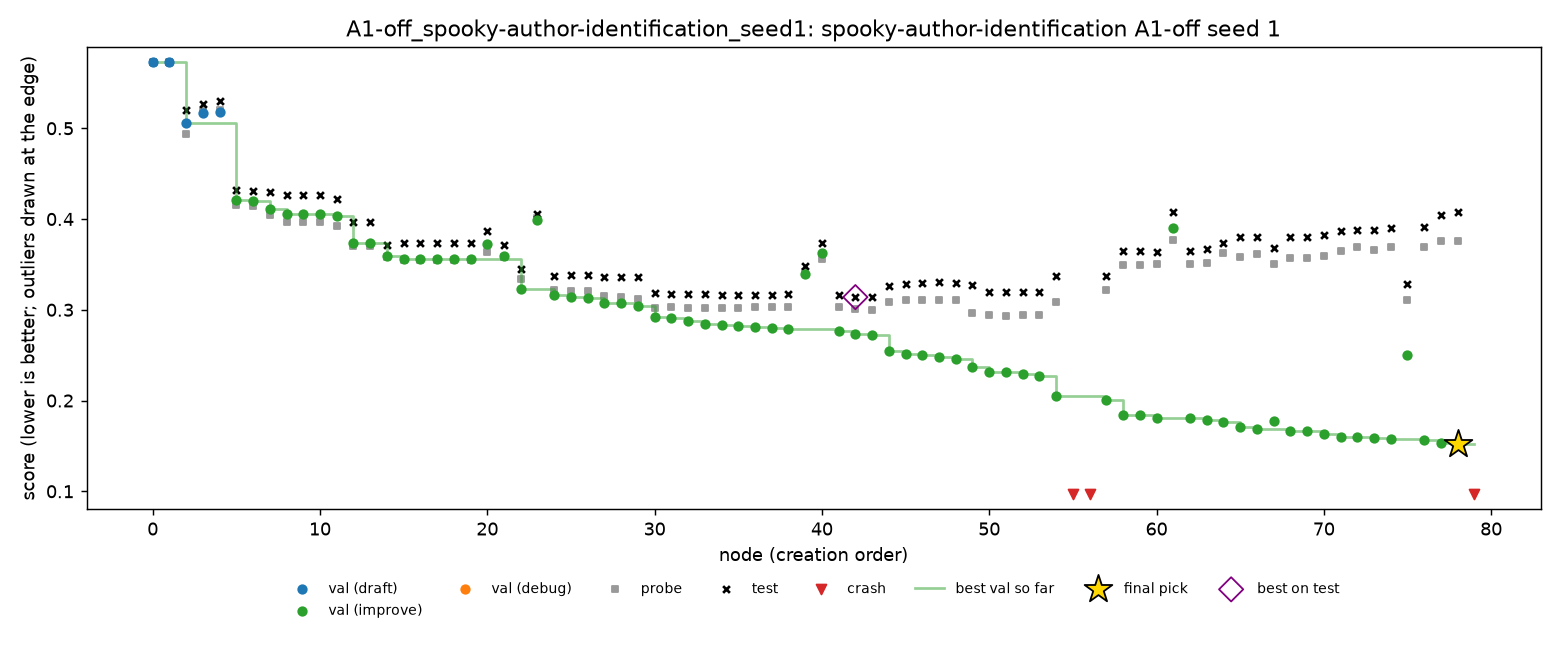
\includegraphics[width=0.6\linewidth]{spooky/analysis/charts/trajectory_A1-off_seed1.png}
\caption{Spooky A1-off seed 1 (log loss): validation (green) falls; probe (grey) and test (black) rise.}
\label{fig:leak}
\end{figure}

\textbf{Case study: a leak.} In spooky A1-off seed 1 the agent stacked models on
its own validation split (Figure~\ref{fig:leak}). Validation fell to 0.152 while probe
and test rose after node 44, ending at 0.408. This is the divergence C4 looks for:
replayed on this run, the rule would have improved the pick to 0.314. With leaf's A1-off run, it is one of the rule's two clear wins,
both leaks that A1 prevents by construction.

\textbf{The model family matters more than the condition.} The 9 best of spooky's 21
runs on test all submitted naive Bayes combined with a linear model; on insults,
refitting boosted trees on the exact features of 9 top nodes (top 3 by validation, probe
and test over the 18 A1-on runs) made all 9 worse; pizza's best runs are tree ensembles. Which
family a run lands on early separates runs more than any condition.

\textbf{Failure modes.} Of 5,381 nodes, 93.6--97.3\% per condition ran; the rest are
runtime errors, timeouts and 38 generation errors with no script, hence 5,343 scripts
(Appendix D). The larger failure is quiet: 63\% of working improve
nodes did not beat their parent and 158 changed no prediction. Of 1,007 findings that claim an effect,
only 61\% are supported by the scores they cite (22--50\% hold on the probe), yet all
are shown to the agent as true, which may be why A4-off does no worse.

\textbf{What a person added (C6).} Five 2-hour sessions ran, one per task except pizza
(Appendix E). No session beat C1's range. People read the dashboard sensibly: one spooky prune matched the
C4 rule exactly, but most prunes removed weak branches (far behind with little time
left, broken, or the wrong model family), which the rule does not look at. Redirects and
injects did not produce the intended change: a redirect chooses which node is worked on,
not what changes, and an injected card was ignored for 20 nodes. On leaf the participant
was unsure when to act and made no intervention. As a design implication rather than a finding, the sessions point to where a person
could add value: task knowledge (spooky stalled without the naive Bayes recipe an expert
would supply), data checks (pizza's \texttt{giver\_username\_if\_known} column leaks
the label, invisible to A1) and a direct instruction channel.

\textbf{Costs.} About \$21 for the 63 text-task runs (\$0.29--0.36 per run), \$4.24
for nomad's 21 and \$1.63 for cactus's 13; the policies added no measurable cost, and the
five C6 sessions took 29 human actions over 10 person-hours (about \$0.12 of API calls
each) for no gain beyond noise. Seed 0 ran slower, before we dropped a provider that cut
off 9\% of its calls.

\textbf{Limitations and risks.} (1) Five seeds for C1, C4 and C5 and three for the
ablations; \cite{aira} recommends ten, as rankings can flip at five. (2) 4 hours instead of 24; \cite{aira} reports
that agents diverge only after about 15 hours, and half of spooky's runs found their pick in
the last 3\% of nodes. (3) One
model, and the in-depth analysis covers only the text tasks; on nomad 4 runs failed on an
unstable machine. (4) Scripted policies are reproducible but not behaviourally faithful,
and C6 is five sessions by group members who knew the agent but were not experts in
the tasks, none on pizza: illustrative, not a user study; an expert might judge more
reliably. (5) Insults and pizza ran without container isolation.
(6) Pizza's data leaks the label (MLE-bench
recommends dropping it); no pick used that column. (7) Spooky seeds 0--2 were resumed from 2 to 4 hours.
(8) None of the 5,343 text-task scripts loaded pretrained weights or downloaded anything,
so every model was trained from scratch on 2 CPUs, a large part of the gap to published
agents (Appendix C). The system
executes generated code, A1's static screen misses leaks it has no rule for (as on
leaf) and any leak in the data itself, and A4's unreliable findings can steer the search.

% ====================
% 7. Reproducibility and responsible practice
% ====================
\section*{7. Reproducibility and Responsible Practice}

\textbf{Reproduction.} The repository's \texttt{README.md} gives setup and launch
instructions; each condition is a YAML file in \texttt{configs/conditions/} over
\texttt{configs/base.yaml}. The model is pinned (\texttt{deepseek/deepseek-v4-flash-0731},
fp8, temperature 0.7, provider routing in the config), and A1's split seed is fixed, so
all A1-on runs on a task share identical splits and harness. Every prompt, completion and
checkpoint is logged; the repository holds each run's grade, outcomes, intervention log
and analysis tables, and \texttt{docs/results/analysis/} regenerates the tables. Raw run
folders contain competition data, so they stay with the members who ran them, available
on request. LLM outputs are not deterministic, so our claims are distributional.

\textbf{Safeguards.} Scripts run in a Docker sandbox with no network, credentials or
host access, except the Kaggle subprocess sandbox noted above. A2 returns only a fixed
card schema from allowlisted documentation, labelled untrusted in A3's prompt
\cite{insthier}; a planted instruction on an allowlisted page never reached generated code
(0 of 8 drafts over two models), which shows the defences held here, not that injection is
impossible. API keys stay in environment variables; C6 participants were group members
and no personal data was collected. MLE-bench tasks are public, which costs twice: A2 must
block solution sites, and the model may have seen solutions in training; tasks whose
solutions are not public would avoid both.

% ====================
% 8. Conclusion
% ====================
\section*{8. Conclusion}

Over 118 controlled runs on six tasks, interventions modelled on a monitoring human did
not improve an interruptible tree-search MLE agent: the validation--test drift they target
barely occurred once evaluation was separated from optimisation, and where held-out data
was small enough for drift to appear, the monitor's signal was too noisy to act on.
Without that separation, 2 of 17 runs leaked. As a design implication, a person may help
most by supplying task knowledge, checking the data, and telling the agent what to change.


% ====================
% End of main text (8-page limit)
% ====================
\clearpage

% ====================
% Contribution statement (not counted toward the page limit)
% ====================
\section*{Contribution Statement}


\begin{center}
\small
\begin{tabular}{@{}>{\raggedright\arraybackslash}p{0.28\linewidth}
                >{\raggedright\arraybackslash}p{0.52\linewidth}
                >{\centering\arraybackslash}p{0.12\linewidth}@{}}
\toprule
\textbf{Member (Student ID)} & \textbf{Main contributions} & \textbf{Share (\%)} \\
\midrule
Nabil Rakaiza Abror (A0305715J) & Proposed the project idea and research question;
  wrote the proposal and work plan and coordinated the role split and run schedule.
  Built the core agent (A3 coding, A5 controller: operators, greedy search, safe points,
  checkpoints and resume, final selection) and A2 retrieval with the prompt-injection
  red team. Integrated all roles (sandbox limits, MLE-bench grading, grid launcher,
  cost and outcome reports, policy replay, merged dashboard, C6 protocol). Ran the
  spooky, insults and pizza full plans (63 runs) and the spooky and insults C6 sessions;
  did the cross-task analysis and compiled all results. & 50 \\
Dziand Dafi Ginandjar (A0354009J) & Built A1 (seeded splits, frozen harness, leakage
  screen, A1-off mode), A4 reflection with evidence-backed findings, and the C5
  finding-correction policy; wrote the leakage stress test, finding-accuracy check, and
  validation--test gap and probe-fidelity analyses. Ran cactus at 2 and 4 hours (26
  runs) and its C6 session, two runs with an LLM monitor (cactus, pizza), and fixed
  pizza's CSV quoting. & 20 \\
Medhini Karthikeyan (A0351868N) & Built the Docker execution sandbox, LLM call
  logging and pilot-run infrastructure, and the ML Docker image. Ran leaf's half plan
  (13 runs) and full plan (21 runs at 4 hours), its C6 session, grading and write-ups.
  & 15 \\
Sahishnav Kritin Karamarathur Senthil Kumar (A0357345X) & Built the C4
  divergence-prune policy and the first version of the monitoring dashboard; fixed the
  coding agent's \texttt{OUTPUT\_DIR} filtering. Ran nomad's half plan (13 runs) and
  full plan (21 runs at 4 hours), its C6 session, and the write-ups. & 15 \\
\midrule
\textbf{Total} & & \textbf{100} \\
\bottomrule
\end{tabular}
\end{center}

% ====================
% References (not counted toward the page limit)
% ====================
\begin{thebibliography}{99}

\bibitem{mlebench}
J.~S. Chan et al.
\newblock MLE-bench: Evaluating Machine Learning Agents on Machine Learning
  Engineering.
\newblock \emph{ICLR}, 2025. arXiv:2410.07095.

\bibitem{aide}
Z.~Jiang, D.~Schmidt, D.~Srikanth, D.~Xu, I.~Kaplan, D.~Jacenko, and Y.~Wu.
\newblock AIDE: AI-Driven Exploration in the Space of Code.
\newblock arXiv:2502.13138, 2025.

\bibitem{aira}
E.~Toledo, K.~Hambardzumyan, M.~Josifoski et al.
\newblock AI Research Agents for Machine Learning: Search, Exploration, and
  Generalization in MLE-bench.
\newblock arXiv:2507.02554, 2025.

\bibitem{mlestar}
J.~Nam, J.~Yoon, J.~Chen, J.~Shin, S.~\"O. Ar{\i}k, and T.~Pfister.
\newblock MLE-STAR: Machine Learning Engineering Agent via Search and Targeted
  Refinement.
\newblock arXiv:2506.15692, 2025.

\bibitem{mlmaster}
Z.~Liu, Y.~Cai, X.~Zhu et al.
\newblock ML-Master: Towards AI-for-AI via Integration of Exploration and Reasoning.
\newblock arXiv:2506.16499, 2025.

\bibitem{mlmaster2}
X.~Zhu, Y.~Cai, Z.~Liu et al.
\newblock Toward Ultra-Long-Horizon Agentic Science: Cognitive Accumulation for
  Machine Learning Engineering.
\newblock arXiv:2601.10402, 2026.

\bibitem{agdebugger}
W.~Epperson et al.
\newblock Interactive Debugging and Steering of Multi-Agent AI Systems.
\newblock \emph{CHI}, 2025.

\bibitem{magentic}
H.~Mozannar et al.
\newblock Magentic-UI: Towards Human-in-the-loop Agentic Systems.
\newblock Microsoft Research, 2025.

\bibitem{react}
S.~Yao, J.~Zhao, D.~Yu, N.~Du, I.~Shafran, K.~Narasimhan, and Y.~Cao.
\newblock ReAct: Synergizing Reasoning and Acting in Language Models.
\newblock \emph{ICLR}, 2023.

\bibitem{tot}
S.~Yao, D.~Yu, J.~Zhao, I.~Shafran, T.~L. Griffiths, Y.~Cao, and K.~Narasimhan.
\newblock Tree of Thoughts: Deliberate Problem Solving with Large Language Models.
\newblock \emph{NeurIPS}, 2023.

\bibitem{sweagent}
J.~Yang, C.~E. Jimenez, A.~Wettig, K.~Lieret, S.~Yao, K.~Narasimhan, and O.~Press.
\newblock SWE-agent: Agent-Computer Interfaces Enable Automated Software
  Engineering.
\newblock \emph{NeurIPS}, 2024.

\bibitem{genagents}
J.~S. Park, J.~C. O'Brien, C.~J. Cai, M.~R. Morris, P.~Liang, and M.~S. Bernstein.
\newblock Generative Agents: Interactive Simulacra of Human Behavior.
\newblock \emph{UIST}, 2023.

\bibitem{insthier}
E.~Wallace, K.~Xiao, R.~Leike, L.~Weng, J.~Heidecke, and A.~Beutel.
\newblock The Instruction Hierarchy: Training LLMs to Prioritize Privileged
  Instructions.
\newblock arXiv:2404.13208, 2024.

\bibitem{deepseek}
DeepSeek-AI.
\newblock DeepSeek V4 Flash (\texttt{deepseek-v4-flash-0731}).
\newblock Large language model, accessed through OpenRouter, 2026.

\bibitem{openrouter}
OpenRouter.
\newblock Unified API for large language models.
\newblock \url{https://openrouter.ai}, accessed November 2026.

\bibitem{docker}
D.~Merkel.
\newblock Docker: Lightweight Linux Containers for Consistent Development and
  Deployment.
\newblock \emph{Linux Journal}, 2014(239), 2014.

\bibitem{streamlit}
Streamlit.
\newblock An open-source Python framework for data apps.
\newblock \url{https://streamlit.io}, accessed November 2026.

\bibitem{sklearn}
F.~Pedregosa et al.
\newblock Scikit-learn: Machine Learning in Python.
\newblock \emph{Journal of Machine Learning Research}, 12:2825--2830, 2011.

\bibitem{pytorch}
A.~Paszke et al.
\newblock PyTorch: An Imperative Style, High-Performance Deep Learning Library.
\newblock \emph{NeurIPS}, 2019.

\bibitem{claude}
Anthropic.
\newblock Claude Opus 5.5.
\newblock Large language model, 2026.

\end{thebibliography}

% ====================
% Appendix (optional, not counted toward the page limit)
% ====================
\appendix
\section*{Appendix}

\subsection*{A. Medals per task}

\begin{table}[H]
\centering
\small
\begin{tabular}{@{}lccc@{}}
\toprule
\textbf{Condition} & \textbf{Spooky} & \textbf{Insults} & \textbf{Pizza} \\
\midrule
C1 & 0 of 5 & 5 gold of 5 & 4 bronze of 5 \\
C4 & 0 of 5 & 5 gold of 5 & 2 bronze of 5 \\
C5 & 1 bronze of 5 & 5 gold of 5 & 1 bronze of 5 \\
A1-off & 0 of 3 & 3 gold of 3 & 1 bronze of 3 \\
A4-off & 0 of 3 & 3 gold of 3 & 1 bronze of 3 \\
\bottomrule
\end{tabular}
\end{table}

\subsection*{B. Other rules for the final pick}

\begin{table}[H]
\centering
\small
\begin{tabular}{@{}lccc@{}}
\toprule
\textbf{Rule} & \textbf{Spooky test (loss)} & \textbf{Insults test (loss)}
& \textbf{Pizza test (loss)} \\
\midrule
Best validation (used) & 0.3284 (0.0009) & 0.9059 (0.0039) & 0.6879 (0.0105) \\
Best probe & 0.3296 (0.0021) & 0.9057 (0.0041) & 0.6790 (0.0195) \\
Validation and probe, row-weighted & 0.3285 (0.0011) & 0.9060 (0.0038) & 0.6868 (0.0117) \\
Mean rank on validation and probe & 0.3286 (0.0012) & 0.9059 (0.0039) & 0.6840 (0.0145) \\
\bottomrule
\end{tabular}
\caption{Means over the 18 A1-on runs per task. ``Loss'' is the distance to the run's
best node on test.}
\end{table}

\subsection*{C. Comparison with published agents}
\label{app:compare}

From the official MLE-bench grading reports of the leaderboard experiments, mean test
score per task. Budgets, hardware and models differ, so this only places our numbers.

\begin{table}[H]
\centering
\small
\begin{tabular}{@{}lccc@{}}
\toprule
\textbf{Agent} & \textbf{Spooky} $\downarrow$ & \textbf{Insults} $\uparrow$
& \textbf{Pizza} $\uparrow$ \\
\midrule
Ours (21 runs, 4 h, DeepSeek V4 Flash) & 0.333 & 0.906 & 0.688 \\
AIDE, GPT-4o, CPU only & 0.498 & 0 of 12 valid & 0.650 \\
AIDE, o1-preview & 0.321 & 0.905 & 0.656 \\
AIRA-dojo, o3 & 0.247 & 0.949 & 0.629 \\
Top entries (Gemini 3 Pro) & $\sim$0.21--0.25 & $\sim$0.955 & $\sim$0.70 \\
\bottomrule
\end{tabular}
\end{table}

\subsection*{D. Node outcomes by condition}

\begin{table}[H]
\centering
\small
\begin{tabular}{@{}lcccccc@{}}
\toprule
\textbf{Condition} & \textbf{Working} & \textbf{Runtime error} & \textbf{Timeout}
& \textbf{Generation error} & \textbf{Leak stop} & \textbf{Pruned} \\
\midrule
C1 & 95.5\% & 2.0\% & 1.7\% & 0.7\% & 2 & 0 \\
C4 & 93.6\% & 2.4\% & 1.5\% & 0.8\% & 0 & 23 \\
C5 & 97.3\% & 0.7\% & 1.3\% & 0.7\% & 0 & 0 \\
A1-off & 95.4\% & 2.6\% & 1.5\% & 0.5\% & 0 & 0 \\
A4-off & 96.0\% & 1.7\% & 1.4\% & 0.7\% & 1 & 0 \\
\bottomrule
\end{tabular}
\caption{5,381 nodes over the 63 runs.}
\end{table}

\subsection*{E. Live human sessions (C6)}

\begin{table}[H]
\centering
\footnotesize
\begin{tabular}{@{}lllll@{}}
\toprule
\textbf{Task} & \textbf{Monitor} & \textbf{Actions} & \textbf{Test (C1's range)} & \textbf{Effect} \\
\midrule
Spooky  & person, 2 h & 9 prune, 2 redirect, correct & 0.368 (0.295--0.390) & none \\
Insults & person, 2 h & 4 prune, 2 redirect, inject, override & 0.9087 (0.901--0.909) & +0.001 \\
Nomad   & person, 2 h & 1 prune & 0.0614 (0.0599--0.0653) & none \\
Cactus  & person + LLM, 2 h & 8 prune & 0.99953 (0.99917--0.99994) & none \\
Leaf    & person, 2 h & none & 0.0261 (0.0128--0.0601) & -- \\
\bottomrule
\end{tabular}
\caption{Live human sessions (C6), one seed each, 2 hours. C1's range is over its seeds,
read from checkpoints at 2 hours where the grid ran 4. ``Person + LLM'': the participant
chose among prunes an LLM assistant suggested. Effect is on the final pick.}
\label{tab:c6}
\end{table}

\subsection*{F. Runs with an LLM monitor (outside the study)}

Two extra 4-hour runs, both on one member's Mac in Docker, used Claude (Opus 5.5)
\cite{claude} as the monitor instead of a person: it read validation and probe scores, plans and scripts
every 15 minutes and queued prunes through the same queue as the dashboard, following
criteria taken from the human cactus session. These are not C6 sessions as the proposal
defines them, and we do not use them in the main analysis.

\begin{table}[H]
\centering
\small
\begin{tabular}{@{}lllll@{}}
\toprule
\textbf{Task} & \textbf{Actions} & \textbf{Test} & \textbf{C1's range (4 h)} & \textbf{Effect on the pick} \\
\midrule
Cactus (seed 102) & 9 prune & 0.99995 & 0.99953--0.99987 & none \\
Pizza (seed 100) & 79 prune & 0.6671 & 0.684--0.709 & worse \\
\bottomrule
\end{tabular}
\end{table}

On cactus every node sits near AUC 0.9999, and the prunes removed only waste. On pizza
the monitor pruned every child that scored below its parent on validation, which on 576
rows is noise: it removed the four best nodes on test and pushed the search into one
line that improved on validation while falling on test. The C4 rule, replayed on the
same run, would have pruned that line and scored 0.6795 (+0.012). A monitor without a
sense of the task's noise can make a run worse. Write-ups:
\texttt{docs/results/\{cactus,pizza\}/c6-4h.md}. The human sessions' notes, intervention
logs and timelines are in \texttt{docs/results/<task>/}.

\subsection*{G. Nomad (full plan, 4 hours)}

\begin{table}[H]
\centering
\small
\begin{tabular}{@{}lcccc@{}}
\toprule
\textbf{Condition} & \textbf{Valid} & \textbf{Mean test RMSLE} $\downarrow$
& \textbf{Medals} & \textbf{Pick's gap (median)} \\
\midrule
C1 & 5 of 5 & 0.06089 & 4 silver, 1 bronze & $-0.0001$ \\
C2 (oracle) & 5 of 5 & 0.06044 & 4 silver, 1 bronze & -- \\
C3 (top 3) & 5 of 5 & 0.06078 & 4 silver, 1 bronze & -- \\
C4 & 5 of 5 & 0.06165 & 4 silver, 1 bronze & $-0.0006$ \\
C5 & 3 of 5 & 0.06146 & 3 silver & $-0.0004$ \\
A1-off & 2 of 3 & 0.06102 & 2 silver & $-0.0047$ \\
A4-off & 2 of 3 & 0.05907 & 2 silver & $-0.0015$ \\
\bottomrule
\end{tabular}
\caption{Nomad, 21 runs; thresholds: median 0.0699, bronze 0.0658, silver 0.0623,
gold 0.0559. Means are over valid runs only. The 4 invalid runs produced no working
node. The gap is oriented as in Table~\ref{tab:claims}: negative means validation was optimistic. From
\texttt{docs/results/nomad/full-4h/}.}
\end{table}

\subsection*{H. Leaf and cactus (4 hours)}

\begin{table}[H]
\centering
\small
\begin{tabular}{@{}lcccc@{}}
\toprule
& \multicolumn{2}{c}{\textbf{Leaf} (log loss $\downarrow$)} & \multicolumn{2}{c}{\textbf{Cactus} (AUC $\uparrow$)} \\
\textbf{Condition} & \textbf{Mean} & \textbf{Medals} & \textbf{Mean} & \textbf{Medals} \\
\midrule
C1 & 0.0849 & 1 silver, 1 bronze & 0.99970 & none \\
C2 (oracle) & 0.0075 & -- & 0.99970 & -- \\
C3 (top 3) & 0.0149 & -- & 0.99970 & -- \\
C4 & 0.1034 & 1 silver & 0.99985 & none \\
C5 & 0.1660 & none & 0.99968 & none \\
A1-off & 5.4541 & 1 bronze & 0.99998 & none \\
A4-off & 0.2428 & 1 gold & 0.99978 & none \\
\bottomrule
\end{tabular}
\caption{Leaf: 21 runs, all valid; thresholds median 0.1083, bronze 0.0153, silver
0.0079, gold 0.0 (A4-off's 0.0 run reached it, as the original leaderboard did). A1-off's mean is driven by one run at 15.66, and three runs in three
conditions scored exactly 0.34888 (and two exactly 0.36408), most likely because every
A1-on run trains on the same split, so runs that end on the same deterministic model
submit identical predictions; we do not have their scripts to confirm it. Cactus: 13 runs (seeds 0--2, ablations 0--1), all
valid and above the median 0.9991; every medal needs AUC 1.0. From
\texttt{docs/results/leaf/full-4h/} and \texttt{docs/results/cactus/4h.md}.}
\end{table}

\subsection*{I. Permissions}

\begin{table}[H]
\centering
\small
\begin{tabular}{@{}lccccc@{}}
\toprule
& \textbf{Read data} & \textbf{Write harness} & \textbf{Execute code}
& \textbf{Web access} & \textbf{Write tree / KB} \\
\midrule
A1 Evaluation  & yes & yes (once) & yes, sandbox & no  & no \\
A2 Retrieval   & no  & no         & no           & allowlisted & model cards only \\
A3 Coding      & yes & \textbf{no}& yes, sandbox & no  & no \\
A4 Reflection  & no  & no         & no           & no  & findings only \\
A5 Controller  & no  & no         & no           & no  & yes \\
Human monitor  & view & no        & no           & no  & via queue only \\
\bottomrule
\end{tabular}
\caption{Permission matrix. A3 cannot modify the harness or reach the network, so it
can neither redefine its objective nor fetch code. On Kaggle (insults, pizza) the
subprocess sandbox does not enforce the network rule.}
\label{tab:perms}
\end{table}

\subsection*{J. Machines}

Spooky: MacBook Pro (M1), Docker. Cactus: MacBook Pro (M2), Docker in Colima. Nomad:
Asus Zenbook A, Windows ARM64 (Snapdragon X X1-26-100), Docker on WSL2. Leaf: HP ENVY
x360 13, Windows x64 (Intel Core i5-1230U), Docker Desktop. Insults and pizza: Kaggle
CPU sessions, subprocess sandbox. Every run: 2 CPUs, CPU-only training.

\end{document}
